\chapter{Visual Recognition}
Pictures are valuable to accurately infer the emotion expressed by a user. For instance, happy photos might contain sunny landscapes or sandy beaches while sad pictures might contain darker colors. To analyse the images, we'll use convolutional neural networks, which achieve state-of-the-art performances in many visual recognition tasks. First we'll explain how they work and then we'll dive into the architecture we've used for deep sentiment analysis.
%%%%%%%%%%%%%%%%%%%%%%%%%%%%%%%%%%%%%%%%%%%%%%%%%%%%%%%%%%%%
%%%%%%%%%%%%%%%%%%%%  NEW SECTION   %%%%%%%%%%%%%%%%%%%%%%%%
%%%%%%%%%%%%%%%%%%%%%%%%%%%%%%%%%%%%%%%%%%%%%%%%%%%%%%%%%%%%
\section{Convolutional Neural Networks}
Convolutional neural networks, often called ConvNets, were inspired by the work of Hubel and Wiesel \cite{hubel} on the human visual cortex. They found that our visual cortex operates as a complex arrangement of cells, where each cell is receptive to a small region of the visual field and is called a {\em receptive field}.

\subsection{Convolutional Layer}
Suppose we have an image of dimension $(h,w,3)$ with $h$ the height, $w$ the width and {\em3} representing the number of channels -- red, blue and green. If we simply flatten that image and transform it into a vector of size $h\times w \times 3$ and feed it to a neural network, we'll get poor results as we've thrown away all the spatial information. Convolutions extract that spatial information and work the following way:
\begin{itemize}
    \item Each convolution is described by a filter F of size $(f, f, 3)$, $f$ usually being equal to 3, 5, or 7.
    \item We position the filter on the upper left side of the image and element-wise multiply the $f\times f \times 3$ chunk of image with the filter. We then sum those 
    numbers to obtain a `neuron'.
    \item We slide across the image, one pixel at a time horizontally and vertically, and repeat the previous operation (see Figure \ref{convolution}).
\end{itemize}

\begin{figure}[H]
\begin{subfigure}[t]{.5\textwidth}
  \vskip 0pt
  \centering
  \includegraphics[width=.8\linewidth]{Images/conv1.png}
  \caption{One operation of convolution}
\end{subfigure}
\begin{subfigure}[t]{.5\textwidth}
  \vskip 0pt 
  \centering
  \includegraphics[width=.8\linewidth]{Images/conv2.png}
  \caption{The result of a convolution}
\end{subfigure}
\caption{A convolution, where each neuron is a `receptive field' \cite{gorner}}
\label{convolution}
\end{figure}

By sliding through the image, we will get a new matrix of dimension $(h_{new}, w_{new})$, with $h_{new}=h-f+1$ and $w_{new}=w-f+1$. However, we usually don't want to reduce the size of our input image that fast, as we want to stack several convolutions. To ensure that the image has the same size after each convolution, zero-padding is used: we add $p$ zeros to the borders of the input image to preserve the spatial size of the input after the convolution (see Figure \ref{fig:zeropadding}).

With zero-padding, $h_{new}$ becomes: $h_{new} =  h + 2p - f + 1$, and we want $h_{new}$ to be equal to $h$, i.e.:
\begin{equation}
    h + 2p - f + 1 = h
    \label{zeropadding}
\end{equation}
Solving (\ref{zeropadding}) gives $p=\frac{f-1}{2}$. 

\begin{figure}[H]
\centering
\includegraphics[width=0.4\textwidth]{Images/zeropadding.png}
\caption{Zero-padding with $p=1$}
\label{fig:zeropadding}
\end{figure}

Zeros are used instead of any other number because we want the filter to activate on the pixels of the image only, therefore, setting the added border to zeros ensures that the resulting neuron will not be influenced by the border.

A convolution directly applied on an image extracts information such as edges or blotches of some color.
\begin{figure}[H]
\centering
\includegraphics[width=0.8\textwidth]{Images/conv_ex.png}
\caption{Examples of convolution}
\label{fig:ex-conv}
\end{figure}

The grayscale and edge filters in Figure \ref{fig:ex-conv} were hardcoded but in a ConvNet setting, the weights of the filter F are learned through optimising a loss function -- in our case, a metric measuring how accurate the predictions of the emotions are. The network will learn weights that will detect features that will be most relevant to our specific task.

A convolution also has a \textbf{depth} parameter $d$: we simply repeat the operation described above $d$ times with $d$ independent filters of the same size $(f, f, 3)$. The $d$ resulting matrices of size $(h,w)$ are then stacked to create a new tensor of dimension $(h,w,d)$.

We can then apply convolutions on that new tensor. First layers will detect simple features such as edges or aggregation of colors, and deeper layers might recognise more complex features such as faces.

\subsection{ReLU Layer}
Stacking convolutions is nice, but as it is, we're only creating features that are linearly dependent on the input pixels: we could in fact replace all the convolutions with a single matrix multiplication. In order to learn more interesting functions, we have to add non-linearities -- that is to say transforming the tensor $(h,w,d)$ with a non-linear function. Historically, the popular choice was the sigmoid function defined as:
\begin{equation}
\text{sigmoid}(x) = \frac{1}{1+e^{-x}}
\end{equation}

\begin{figure}[H]
\centering
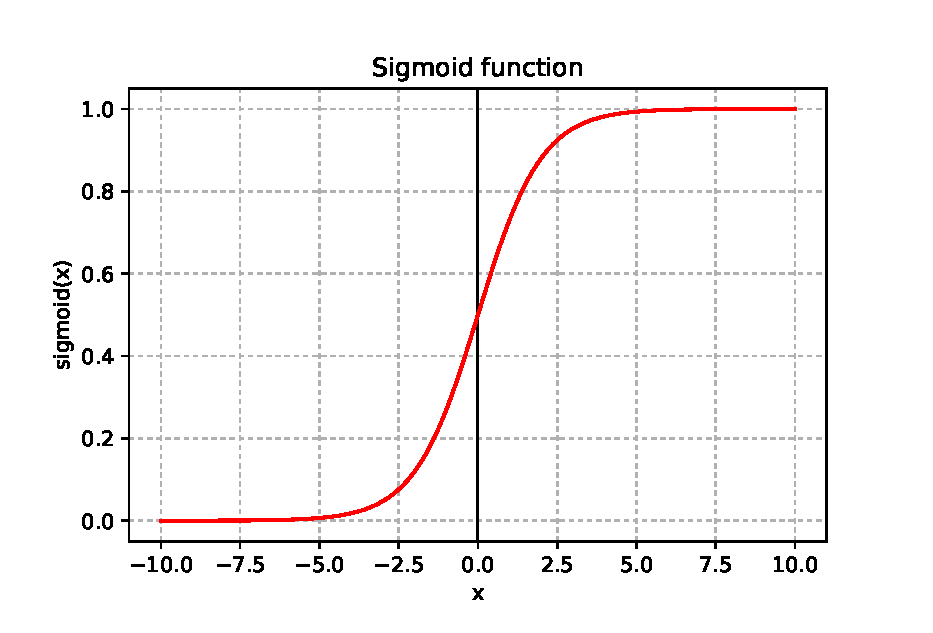
\includegraphics[width=0.5\textwidth]{Images/sigmoid.eps}
\caption{Sigmoid function}
\end{figure}

The sigmoid function is the simplest function to have values between 0 and 1, mimicking the biological neurons `firing' in reaction to their inputs. However, when the network is learning to minimise a loss function through backpropagation, the gradients tend to vanish to zero as the sigmoid's derivative goes to zero for values that are highly negative or positive. The most popular choice of non-linearity is now the Rectified Linear Unit (ReLU) \cite{nair} defined as:
\begin{equation}
\text{ReLU}(x) = \text{max}(0,x)
\end{equation}

\begin{figure}[H]
\centering
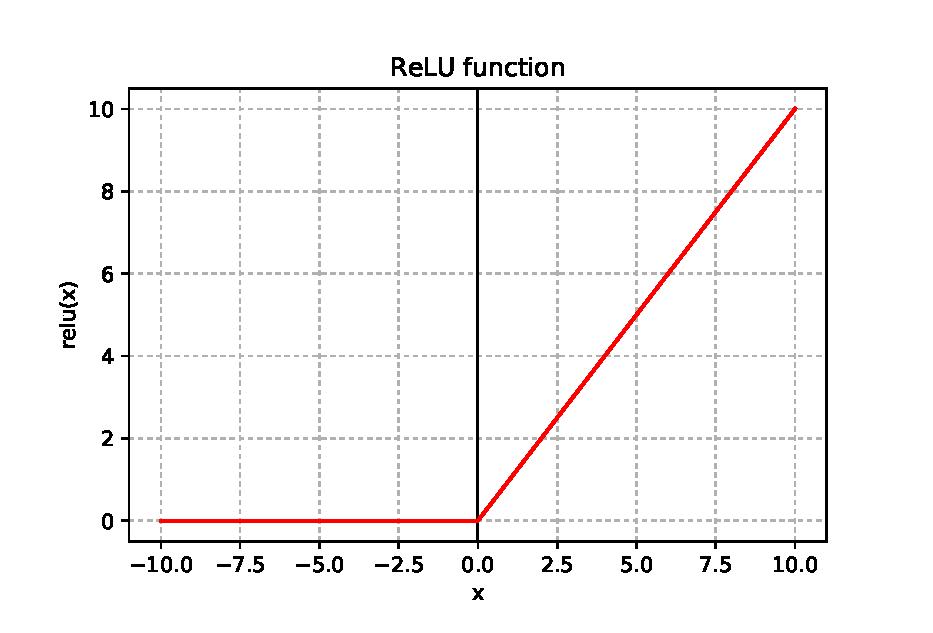
\includegraphics[width=0.5\textwidth]{Images/relu.eps}
\caption{ReLU function}
\end{figure}

The ReLU's gradient is non-saturating for highly excited neurons which turns out to be a nice property to learn faster. In a neural network, each layer of convolution is followed by a ReLU layer, that simply applies the function $\text{max}(0,x)$ to each neuron.

\newpage
\subsection{Pooling Layer}
There is a lot of spatial redundancy in an image, we don't need all the pixels to be able to identify what's in a picture. For example we can perfectly identify the animal in Figure \ref{kittens} by reducing the number of pixels by two.

\begin{figure}[H]
\centering
\includegraphics[width=0.8\textwidth]{Images/kittens.png}
\caption{A kitten, and the same kitten with half the pixels}
\label{kittens}
\end{figure}

The same idea applies to convolved images, we might not need all the neurons that were created. The pooling operation downsamples the image in the following way:
\begin{itemize}
    \item We pick a channel among the $d$ ones.
    \item We start at the top-left $2\times 2$ square of the image and keep the maximum value.
    \item We repeat by sliding through the image vertically and horizontally with a stride of 2 (see Figure \ref{maxpool}).
\end{itemize}

\begin{figure}[H]
\centering
\includegraphics[width=0.8\textwidth]{Images/maxpool.png}
\caption{Max pooling \cite{camb-spark}}
\label{maxpool}
\end{figure}

After applying max pooling to each channel, the resulting image dimension is $(\frac{h}{2}, \frac{w}{2}, d)$ and we have discarded 75\% of the neurons (as in each max-pool operation, we only keep the maximum neuron among the fours), effectively reducing the number of parameters and controlling overfitting.

One could wonder why max-pooling and not average pooling (taking the mean value of the four neurons). The convolutions allow us to see if a certain feature is in the image when a neuron fires, and we only want to know if that feature is there in a certain region. Therefore taking the max of the four neurons is sufficient to know whether that feature is there or not in that particular region.

In practice, after a few iterations of convolutions, inserting pooling layers in-between convolutional layers might be a good idea to control the spatial complexity of the network.

\subsection{An Example of Convolutional Network}
Figure \ref{ex-convnet} shows an example of a convolutional neural network with an input image of size $(224, 224, 3)$:

\begin{figure}[H]
\centering
\includegraphics[width=0.8\textwidth]{Images/conv_archi.png}
\caption{The architecture of a convolutional neural network \cite{gorner}}
\label{ex-convnet}
\end{figure}

We have:
\begin{itemize}
    \item A first convolution with a filter of size $3\times3$, with depth 4, stride 1 and zero-padding of 1.
    \item A ReLU layer.
    \item A second convolution with a filter of size $5\times5$, with depth 8, stride 1 and zero-padding of 2.
    \item A ReLU layer.
    \item Max-pooling of size $2\times2$ with stride 2, reducing the height and width by a factor of 2.
\end{itemize}

After the last operation, the neurons are flatten into a vector that can be fed to more traditional fully connected layers.

\section{Deep Convolutional Networks}
Best results on visual recognition are achieved using deep convolutional networks, that is to say by stacking many layers of convolutions/ReLU/max-pool. But what exactly is `many'? Let us have a look at the winners of the main Computer Vision competition: ImageNet Large Scale Visual Recognition (ILSVR).
\begin{enumerate}
    \item \textbf{AlexNet} \cite{alexnet}: The first popular convolutional network, developed by A. Krizhevsky, I. Sutskever and G. Hinton, that outperformed 
    the other competitors at ILSVR 2012 by a large margin: top-5 error of 16\% compared to the runner-up with 26\%. AlexNet has 5 convolutional layers (followed by 
    ReLU), 3 max-pool layers and 3 fully-connected layers, producing a 8 layers deep network (not counting the max-pooling as it doesn't have any parameters).
    \item \textbf{GoogLeNet} (also known as Inception)\cite{googlenet}: The winner of ILSVR 2014 with a top-5 error of 6.7\% . This 22-layer architecture used 
    the `Inception Module' (that will be described shortly) which allowed to drastically reduce the number of parameters: from 60M for AlexNet to 4M for GoogLeNet.
    \item \textbf{ResNet} \cite{resnet}: The winner of ILSVR 2015 with a top-5 error of 3.6\% thanks to an astonishing 152 layers convolutional network. This 
    architecture features `skip connections' that were decisive for this ultra-deep network to achieve such results.
\end{enumerate}

\section{Transfer Learning}
Training a convolutional network from scratch can be difficult as a large amount of data is needed and plenty of different architectures and hyperparameters need to be tried before finding a decent model. To circumvent that issue, we can take advantage of the pre-trained models available that learned to recognise images through near 1.2M training examples from the ImageNet dataset, and with a deep architecture that took weeks to train on multiple GPUs.

More specifically, the pre-trained networks learned to recognise features in a picture in order to classify the latter among the 1000 classes in the ImageNet dataset. Those features are combined in the final output layer (of size 1000, each neuron being a class probability). Suppose that instead of classifying an image into 1000 classes we want to label it according to 6 different emotions (happy, sad, angry, scared, surprised, disgusted). The same features can be combined in a different way to let the network take a decision about what the emotion conveyed by the image is.

The process described above is called {\em Transfer Learning}: we chop off the last layer of the network and add our own layer given how many classes we have. We then freeze the weights of the other layers and only backpropagate through the newly created layer when training the network on our examples. If we have enough data, we can unfreeze more higher-level layers and backpropagate through them.

Earlier features of ConvNets contain more generic features (such as edges or color blobs) that can be used for any task, while later features become more specific to the details of the classes present in the dataset. For example in ImageNet, there are many dog breeds and the later representational power might be used to distinguish those \cite{transfer}. We will be using Google's Inception network and fine-tune through the last 3 layers.

\section{Google Inception Network}

\subsection{Motivation}
After AlexNet proved that convolutional networks outperformed traditional machine learning models, the trend to achieve even better results was to build wider (more units per layer) and deeper (more layers) networks and to add dropout to address overfitting. However, bigger networks are more expensive to train (more parameters) and could not be usable for real-time prediction if a forward-pass takes too long. Moreover, if the increased capacity is not used efficiently, for example if most added weights are close to zero, then the extra depth and width will be completely wasted.

To address this problem, we could replace the fully connected layers by sparse ones, even inside convolutions \cite{googlenet}. Not only would it mimic more closely biological systems, but it would also have more theoretical ground thanks to the work of S. Arora et al. \cite{arora}. They proved that if the probability distribution of a dataset can be represented by a large, very sparse neural network, then it's possible to build the optimal network layer after layer by clustering highly correlated neurons of the preceding layer. By clustering, they mean grouping neurons into a single entity, by assigning weights to the neurons of the group, that will be fed to the next layer.
This process also resonates well with the Hebbian principle: {\em neurons that fire together, wire together} \cite{hebbian}.

Current network architectures are not using sparse layers as the libraries are heavily optimised for dense matrix multiplication. Training sparse layers would incur considerable overhead (lookups, cache) that are not handled by today's computing infrastructures. However, the Inception module is an elegant solution to add more expressiveness to a network by mimicking sparsity, while keeping the number of parameters low. 

\subsection{Inception Module}
At each layer, we would normally be facing the dilemma of choosing between $1\times 1$, $3\times 3$, $5\times5$ convolution or max-pooling:

\begin{figure}[H]
    \centering
    \includegraphics[width=0.8\textwidth]{Images/inceptionmodule.png}
    \caption{Which layer to choose? \cite{inceptionmodule}}
\end{figure}

In the Inception module, we perform all of the above operations and let the network decide for us. Each operation is done in parallel before being concatenated and fed to the next layer. This allows to capture both local features via small convolutions and more high-level features via large convolutions. 

\begin{figure}[H]
    \centering
    \includegraphics[width=0.8\textwidth]{Images/naiveinception.png}
    \caption{Naive Inception module \cite{googlenet}}
\end{figure}

As it is, the Inception module seems to rather increase the number of parameters. But this is actually the naive implementation of the module. One key component are the $1\times 1$ convolutions, which behave like clustering the highly correlated neurons, before the large convolutions:
\begin{figure}[H]
    \centering
    \includegraphics[width=0.8\textwidth]{Images/inception.png}
    \caption{Inception module \cite{googlenet}}
\end{figure}

Let us take an example to understand how those $1\times 1$ convolutions reduce the number of parameters: suppose at an arbitrary layer, our input size is $(14, 14, 480)$.
\begin{itemize}
\item A \textbf{$\mathbf{5\times 5}$ convolution, depth 48}: requires $(14^2)(480)(5^2)(48) = 112,896,000$ operations (supposing stride 1 and zero-padding).
\item An \textbf{$\mathbf{1\times 1}$ convolution, depth 16, followed by a $\mathbf{5\times 5}$ convolution, depth 48:} requires $[(14^2)(480)(1^2)(16)] + [(14^2)(16)(5^2)(48)] = 5,268,480$ operations.
\end{itemize}

The second operation with $1\times 1$ convolution is more than twenty times faster! The number of parameters is also reduced by twenty as the reduction factor is the same (to get the actual number of parameters, we only need to divide the above by $14^2)$.

\subsection{GoogleNet}
The complete GoogleNet architecture is:

\begin{figure}[H]
    \centering
    \includegraphics[width=\textwidth]{Images/googlenet.png}
    \caption{GoogleNet architecture\cite{googlenet}}
\end{figure}

The `\#$3\times3$ reduce' and `\#$5\times5$ reduce' refer to the dimensionality reduction with the $1\times1$ convolution. The `pool proj' refers to the depth of the $1\times1$ convolution following the $3\times3$ max-pool with stride 1 and zero-padding 1.

In our model, we got rid of the last linear layer and replaced it with another linear layer of size $1 \times 1 \times 6$ for the 6 different emotions.

\newpage
\section{Results}
Are the images enough to infer the emotion conveyed by a user? The Inception model was fed raw images, that were resized to a fixed size $(224, 224, 3)$, and fine-tuned with the following parameters:
\begin{itemize}[topsep=0pt]
    \itemsep-1em
    \item 9,000 training steps
    \item Mini-batch of size 32
    \item Adam optimizer with a learning rate of $1\mathrm{e}{-6}$
\end{itemize}

After the preprocessing described in Section 2, the dataset contains 295,508 posts that we split as 80\% train set and 20\% test set. The metric used to evaluate the model is accuracy, which is the fraction of correctly classified images.

The training process of the Inception fine-tuning was monitored thanks to Tensorboard:
\begin{figure}[H]
    \centering
    \includegraphics[width=\textwidth]{Images/image_model_loss_cleaned.jpg}
    \caption{Loss function of the Inception fine-tuned model}
\end{figure}

\begin{figure}[H]
    \centering
    \includegraphics[width=\textwidth]{Images/image_model_accuracies_cleaned.jpg}
    \caption{Train/validation accuracies of the Inception fine-tuned model}
\end{figure}

The fine-tuned Inception is compared to a baseline: random guessing. Actually this guessing includes the prior probabilities of the classes: 
\begin{table}[H]
\begin{center}
    \begin{tabular}{| c | c | c | c | c | c | c |}
    \hline
     & \textbf{happiness} & \textbf{sadness} &  \textbf{anger} & \textbf{surprise} & \textbf{fear} & \textbf{disgust} \\ \hline
    \textbf{Prior proba.} & 0.32 & 0.22 & 0.19 & 0.03 & 0.22 & 0.02 \\
    \hline
    \end{tabular}
\end{center} 
\caption{Prior probabilities of the classes}
\end{table}

The results are:
\begin{table}[H]
\begin{center}
    \begin{tabular}{| l | c | c |}
    \hline
    & \textbf{Train} & \textbf{Test} \\
    & \textbf{accuracy} & \textbf{accuracy} \\ \hline
    \textbf{Random guessing} & 24\% & 24\% \\ \hline
    \textbf{Inception fine-tuned}  & 48\% & 42\% \\
    \hline
    \end{tabular}
\end{center} 
\caption{Comparison of models using raw images}
\end{table}

The image model is quite satisfactory as even if some images are easy to read:

\begin{figure}[H]
    \centering
    \includegraphics[width=0.8\textwidth]{Images/happy_easy.jpg}
    \caption{Easy to read happy images}
\end{figure}

Some other images are more challenging:

\begin{figure}[H]
    \centering
    \includegraphics[width=0.8\textwidth]{Images/happy_hard.jpg}
    \caption{Harder to read happy images}
\end{figure}




